\documentclass{article}
\usepackage[T1]{fontenc}
\usepackage[utf8]{inputenc}
\usepackage[polish]{babel}
\usepackage{amsmath}
\usepackage{url}
\usepackage{graphicx}
 \usepackage{float}
 \usepackage{pgfplots}
\pgfplotsset{compat=1.18}
%{Informatyka stosowana 2022, I st., semestr VI}


\author{
	{Dominik Gałkowski, 247659} \\
	{Jan Śladowski, 247806}\\ 
{Prowadzący: dr inż. Marcin Kacprowicz}
}

\title{Komputerowe systemy rozpoznawania 2024/2025\\Projekt 2. Podsumowania lingwistyczne relacyjnych baz danych}
\begin{document}
\maketitle 

\section{Cel}
Celem projektu jest stworzenie aplikacji, której główną funkcjonalnością
jest lingwistyczna agregacja zawartości wybranego zbioru danych. Ma ona za zadanie generowanie podsumowań lingwistycznych dla wybranych przez użytkownika kwantyfikatorów, sumaryzatorów i kwalifikatorów dla różnych atrybutów. Analiza otrzymanych wyników polega na określeniu, znaczenia wybranych kwantyfikatorów, sumaryzatorów, kwalifikatorów oraz miar ich jakości dla wiarygodności i jakości otrzymanych podsumowań lingwistycznych. Przykładowe podsumowanie to, np. większość pomiarów ma wysokie ciśnienie.


\section{Baza danych, zmienne lingwistyczne, kwantyfikatory lingwistyczne}

\subsection{Charakterystyka podsumowywanej bazy danych}
W tym projekcie został wykorzystany zbiór danych zapisany w pliku w formacie .csv, na podstawie którego utworzono bazę danych - PostgresSQL. Baza danych o nazwie World Weather Repository zawiera różnego rodzaju pomiary danych atmosferycznych, np. temperatura lub prędkość wiatru. \cite{baza} Użteczność bazy jest określona na stronie Kaggle jako 10.0, a dane z niej są wykorzystywane do prognozowanie pogody oraz analizy klimatu na różnych kontynentach. Baza jest nabieżąco aktualizowana, natomiast na dzień 18.05.2025r. składa się z 71331 rekordów. 

Zmiennym lingwistycznym przypisuje się znaczenie ze względu na potrzebę lepszej interpretowalności danych przez użytkowników. Ludzie rzadko reagują na dokładne wartości (np. 1033.8 mb ciśnienia), natomiast określenie „wysokie ciśnienie” pozwala im intuicyjnie rozumieć sytuację pogodową. Stąd istnieje zapotrzebowanie na „przekładanie” danych formalnych na język naturalny. \\
Podmiotem podsumowań jest pomiar atmosferyczny, z bazy World Weather Repository wybrano 10 atrybutów, które zostaną rozmyte, są to następujące kolumny:
\begin{enumerate}
    \item last\_updated - data przeprowadzenia pomiarów, z tego atrybutu zostanie wykorzystana godzina w celu określenia pory dnia, zakres [0 - 24]. 
    \item temperature\_celsius - temperatura wyrażona w stopniach Celsjusza w zakresie [-25, 50].
    \item wind\_kph - prędkość wiatru wyrażona w kilometrach na godzinę w zakresie [3, 151]. 
    \item pressure\_mb - ciśnienie powietrza wyrażone w milibarach w zakresie [947 - 1050]. 
    \item humidity - wilgotność w zakresie [2 - 100\%].
    \item visibility\_km - widoczność wyrażona w kilometrach w zakresie [0, 32].
    \item uv\_index - wartość promieniowania słonecznego UVI w zakresie [0, 16].
    \item air\_quality\_Carbon\_Monoxide - pomiar jakości powietrza ze względu na stężenie tlenku węgla, wyrażony w ppm(liczba cząstek CO2 w milionie cząstek powietrza), w zakresie [0 - 2220].
    \item air\_quality\_Nitrogen\_dioxide - pomiar jakości powietrza ze względu na stężenie dwutlenku azotu, wyrażony w ppm(liczba cząstek NO2 w milionie cząstek powietrza) w zakresie [0 - 428].
    \item air\_quality\_gb-defra-index - skala określająca poziomy zanieczyszczenia w powietrzu w zakresie [1 - 10].

    
\end{enumerate}

\subsection{Zmienne lingwistyczne (atrybuty/własności obiektów)}
Poniżej zostały zaprezentowane zmienne lingwistyczne dla atrybutów opisanych w sekcji 2.1, ich wzory analityczne oraz wykresy funkcji przynależności wraz z dopasowanymi do nich etykietami. W każdym z poniższych wzorów \(L_x\) to zmienna ligwistyczna, $\mathcal{L}_x$ - nazwa zmiennej lingwistycznej , \(H_x\) zbiór możliwych przyjmowanych wartości, \(X_x\) - przestrzeń rozważań, \(x\) - numer kolejnej zmiennej ligwistycznej. 
\begin{enumerate}
    \item last\_updated
        \begin{equation}
            L_1 = \langle \mathcal{L}_1, H_1, \mathcal{X}_1 \rangle
        \end{equation}
        gdzie: $\mathcal{L}_1$ – pora dnia, $H_1$ – \{nocna, poranna, południowa, popołudniowa, wieczorna\}, $\mathcal{X}_1 = [0, 24]$. \\
        Poniżej wzory dla wszystkich możliwych etykiet.
        \begin{equation}
            \mu_{\text{nocna}}(x) =
            \begin{cases}
            \frac{7 - x}{3}, & x \in (4, 7) \\
            1, & x \in [0, 4] \\
            \frac{x - 21}{3}, & x \in [21, 24) \\
            0, & \text{w przeciwnym razie} \\
            \end{cases}
        \end{equation}

        \begin{equation}
            \mu_{\text{poranna}}(x) =
            \begin{cases}
            \frac{x - 4}{3}, & x \in (4, 7) \\
            1, & x \in [7, 9] \\
            \frac{12 - x}{3}, & x \in (9, 12) \\
            0, & \text{w przeciwnym razie} \\
            \end{cases}
        \end{equation}

        \begin{equation}
            \mu_{\text{południowa}}(x) =
            \begin{cases}
            \frac{x - 9}{3}, & x \in (9, 12) \\
            1, & x \in [12, 13] \\
            \frac{16 - x}{3}, & x \in (13, 16) \\
            0, & \text{w przeciwnym razie} \\
            \end{cases}
        \end{equation}

        \begin{equation}
            \mu_{\text{popołudniowa}}(x) =
            \begin{cases}
            \frac{x - 13}{3}, & x \in (13, 16) \\
            1, & x \in [16, 17] \\
            \frac{20 - x}{3}, & x \in (17, 20) \\
            0, & \text{w przeciwnym razie} \\
             \end{cases}
        \end{equation}

        \begin{equation}
            \mu_{\text{wieczorna}}(x) =
            \begin{cases}
            \frac{x - 17}{3}, & x \in (17, 20) \\
            1, & x \in [20, 21] \\
            \frac{24 - x}{3}, & x \in (21, 24) \\
            0, & \text{w przeciwnym razie} \\
            \end{cases}
        \end{equation} 
        
    \begin{figure}[H]
    \centering
    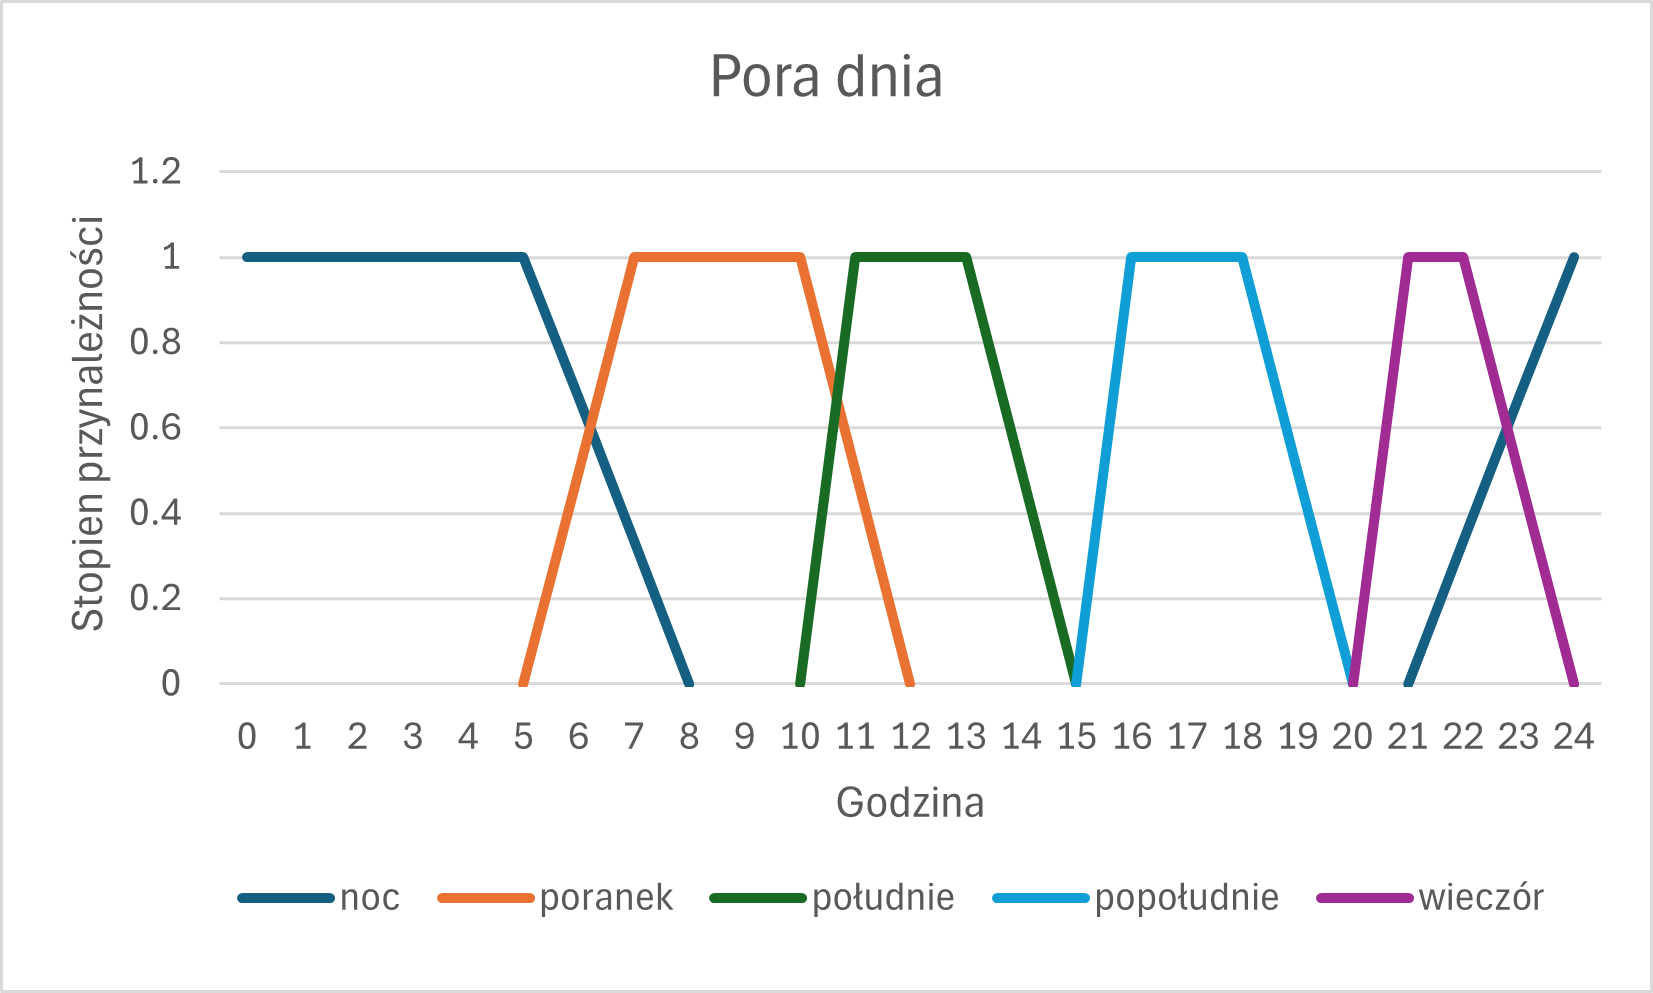
\includegraphics[width=\textwidth]{img/day.png}
    \caption{Wykres funkcji przynależności dla pory dnia.}
    \end{figure}
    
    \item temperature\_celsius
        \begin{equation}
            L_2 = \langle \mathcal{L}_2, H_2, \mathcal{X}_2 \rangle
        \end{equation}
        gdzie: $\mathcal{L}_2$ – temperatura, $H_2$ – \{bardzo zimna, zimna, umiarkowana, ciepła, gorąca\}, $\mathcal{X}_2 = [-25, 50]$. \\
        Poniżej wzory dla wszystkich możliwych etykiet.
                \begin{equation}
                   \mu_{\text{bardzo\_zimna}}(x) =
                    \begin{cases}
                    1, & x \in [-25, -15] \\
                    \frac{-5 - x}{10}, & x \in (-15, -5) \\
                    0, & \text{w przeciwnym razie}
                    \end{cases}
                \end{equation}
                
                \begin{equation}
                   \mu_{\text{zimna}}(x) =
                    \begin{cases}
                    \frac{x + 10}{10}, & x \in (-15, -5) \\
                    1, & x \in [-5, 0] \\
                    \frac{10 - x}{10}, & x \in (0, 10) \\
                    0, & \text{w przeciwnym razie}
                    \end{cases}
                \end{equation}

                \begin{equation}
                    \mu_{\text{umiarkowana}}(x) =
                    \begin{cases}
                    \frac{x}{10}, & x \in (0, 10) \\
                    1, & x \in [10, 15] \\
                    \frac{20 - x}{10}, & x \in (15, 25) \\
                    0, & \text{w przeciwnym razie}
                    \end{cases}
                \end{equation}

                \begin{equation}
                    \mu_{\text{ciepła}}(x) =
                    \begin{cases}
                    \frac{x - 15}{10}, & x \in (15, 25) \\
                    1, & x \in [25, 30] \\
                    \frac{30 - x}{10}, & x \in (30, 40) \\
                    0, & \text{w przeciwnym razie}
                    \end{cases}
                \end{equation}

                \begin{equation}
                    \mu_{\text{gorąca}}(x) =
                    \begin{cases}
                    \frac{x - 30}{10}, & x \in (30, 40] \\
                    1, & x \in 40, 50] \\
                    0, & \text{w przeciwnym razie}
                    \end{cases}
                \end{equation}

        \begin{figure}[H]
    \centering
    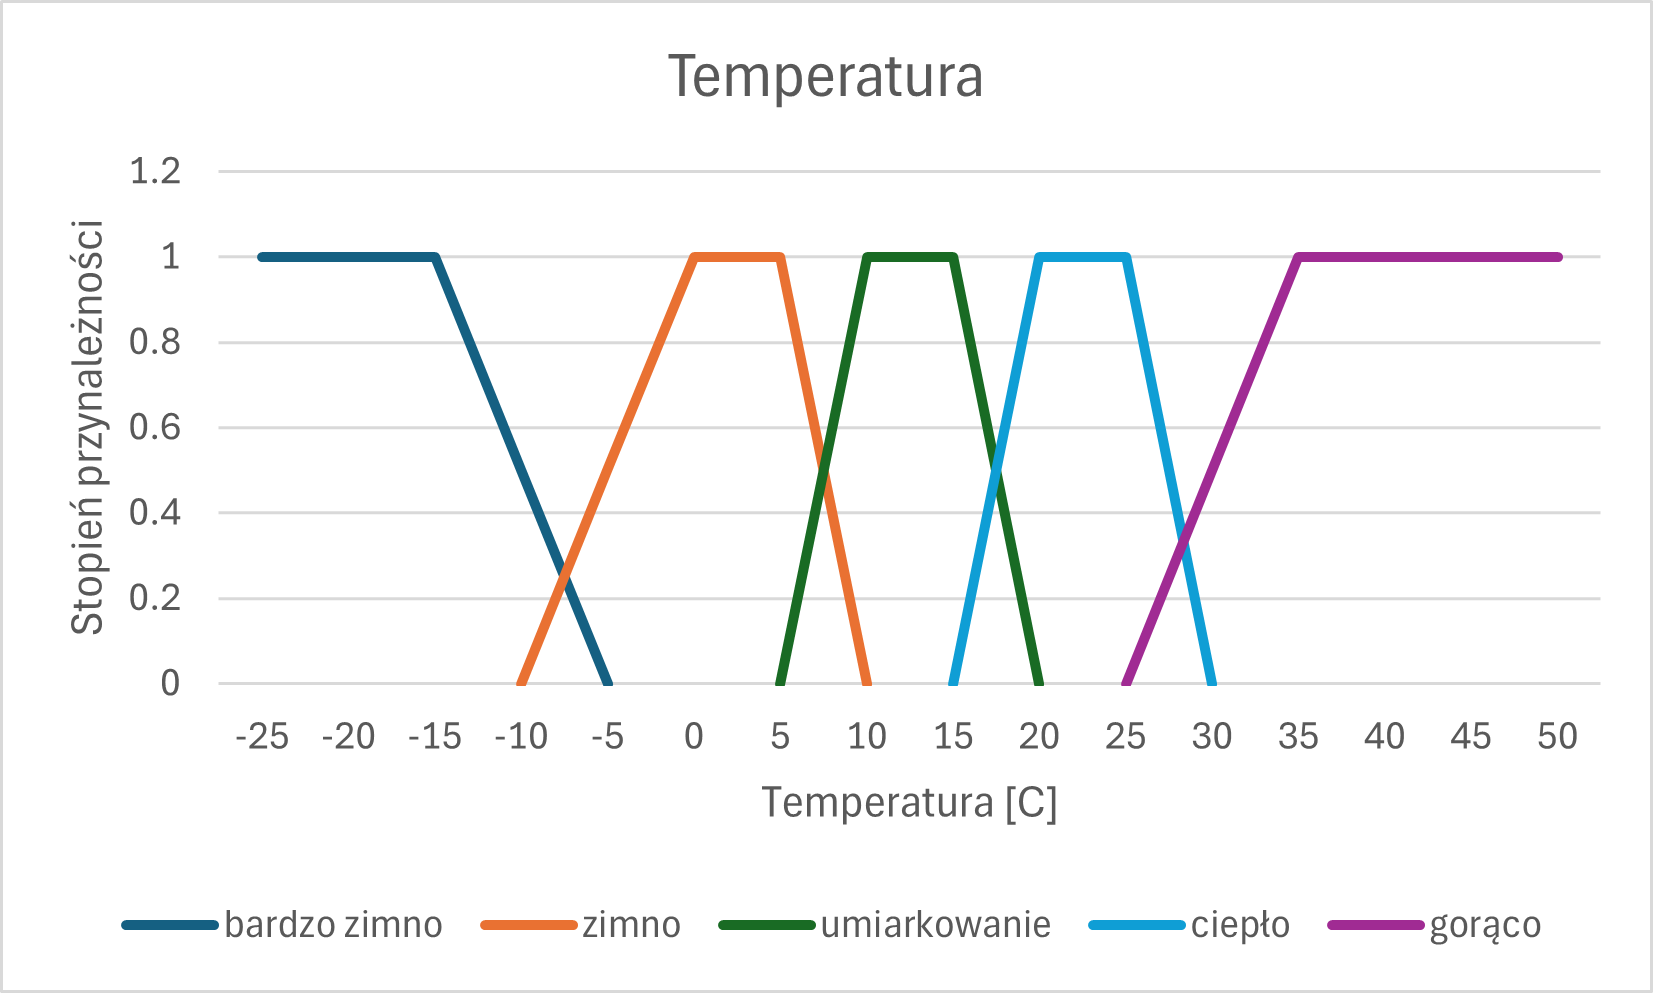
\includegraphics[width=\textwidth]{img/temp.png}
    \caption{Wykres funkcji przynależności dla temperatury.}
    \end{figure}

    \item wind\_kph
        \begin{equation}
            L_3 = \langle \mathcal{L}_3, H_3, \mathcal{X}_3 \rangle
        \end{equation}
        gdzie: $\mathcal{L}_3$ – wiatr, $H_3$ – \{słaby, umiarkowany, silny, bardzo silny, gwałtowny, huragan\}, $\mathcal{X}_3 = [3, 151]$. \\
        Poniżej wzory dla wszystkich możliwych etykiet.
                  \begin{equation}
                    \mu_{\text{słaby}}(x) =
                    \begin{cases}
                    1, & x = 0 \\
                    \frac{20 - x}{20}, & x \in (0, 20) \\
                    0, & \text{w przeciwnym razie}
                    \end{cases}
                  \end{equation}
                \begin{equation}
                    \mu_{\text{umiarkowany}}(x) =
                    \begin{cases}
                    \frac{x}{20}, & x \in (0, 20) \\
                    1, & x = 20 \\
                    \frac{40 - x}{20}, & x \in (20, 40) \\
                    0, & \text{w przeciwnym razie}
                    \end{cases}
                  \end{equation}
                \begin{equation}
                    \mu_{\text{silny}}(x) =
                    \begin{cases}
                    \frac{x - 20}{20}, & x \in (20, 40) \\
                    1, & x = 40 \\
                    \frac{60 - x}{20}, & x \in (40, 60) \\
                    0, & \text{w przeciwnym razie}
                    \end{cases}
              \end{equation}
                \begin{equation}
                    \mu_{\text{bardzo\_silny}}(x) =
                    \begin{cases}
                    \frac{x - 40}{20}, & x \in (40, 60) \\
                    1, & x = 60 \\
                    \frac{80 - x}{20}, & x \in (60, 80) \\
                    0, & \text{w przeciwnym razie}
                    \end{cases}
              \end{equation}
              \begin{equation}
                    \mu_{\text{gwałtowny}}(x) =
                    \begin{cases}
                    \frac{x - 60}{20}, & x \in (60, 80) \\
                    1, & x = 80 \\
                    0, & \text{w przeciwnym razie}
                    \end{cases}
              \end{equation}
                 \begin{equation}
                    \mu_{\text{huragan}}(x) =
                    \begin{cases}
                    \frac{x - 80}{20}, & x \in (80, 100) \\
                    1, & x \in (100, 151) \\
                    0, & \text{w przeciwnym razie}
                    \end{cases}
              \end{equation}
        \begin{figure}[H]
    \centering
    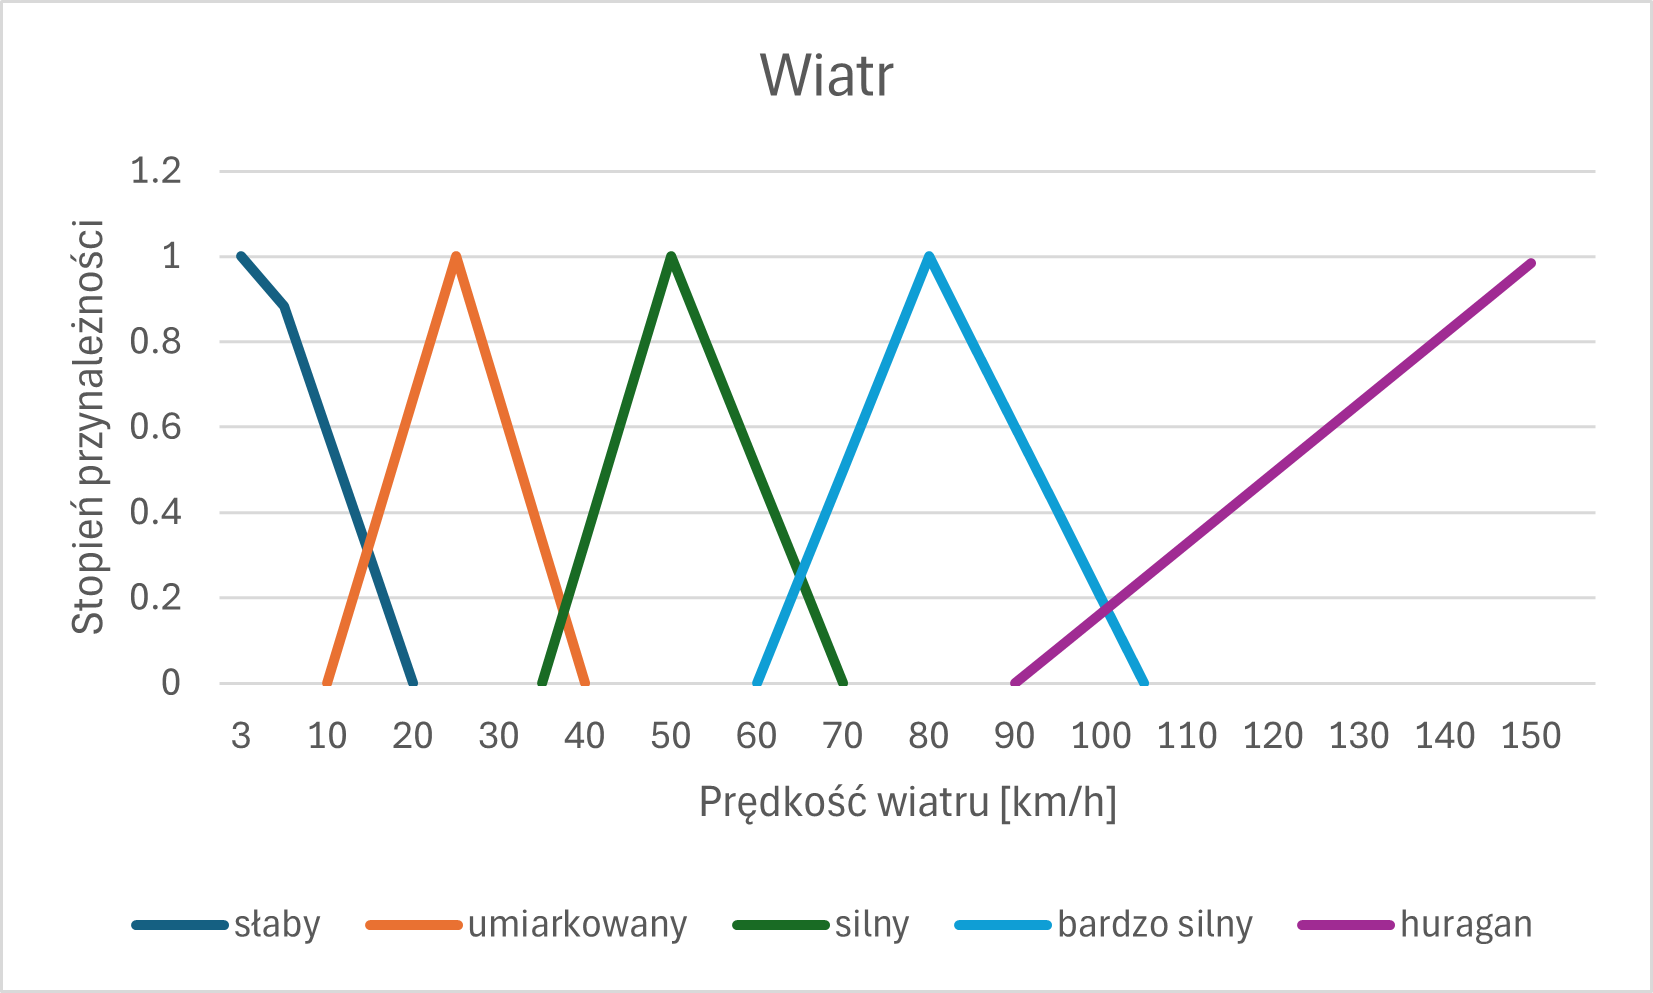
\includegraphics[width=\textwidth]{img/wind.png}
    \caption{Wykres funkcji przynależności dla siły wiatru.}
    \end{figure}
              
    \item pressure\_mb
        \begin{equation}
            L_4 = \langle \mathcal{L}_4, H_4, \mathcal{X}_4 \rangle
        \end{equation}
        gdzie: $\mathcal{L}_4$ – ciśnienie, $H_4$ – \{niskie, normalne, wysokie\}, $\mathcal{X}_4 = [947, 1050]$. \\
        Poniżej wzory dla wszystkich możliwych etykiet.
                \begin{equation}
                    \mu_{\text{niskie}}(x) =
                    \begin{cases}
                    1, & x \in [947, 970] \\
                    \frac{1000 - x}{30}, & x \in (970, 1000] \\
                    0, & \text{w przeciwnym razie}
                    \end{cases}
              \end{equation}
                \begin{equation}
                   \mu_{\text{normalne}}(x) =
                    \begin{cases}
                    \frac{x - 970}{30}, & x \in (970, 1000] \\
                    1, & x \in (1000, 1020] \\
                    \frac{1040 - x}{20}, & x \in (1020, 1040] \\
                    0, & \text{w przeciwnym razie}
                    \end{cases}
                \end{equation}

                \begin{equation}
                \mu_{\text{wysokie}}(x) =
                    \begin{cases}
                    \frac{x - 1020}{20}, & x \in (1020, 1040] \\
                    1, & x \in (1040, 1050] \\
                    0, & \text{w przeciwnym razie}
                    \end{cases}
                \end{equation}

    \begin{figure}[H]
    \centering
    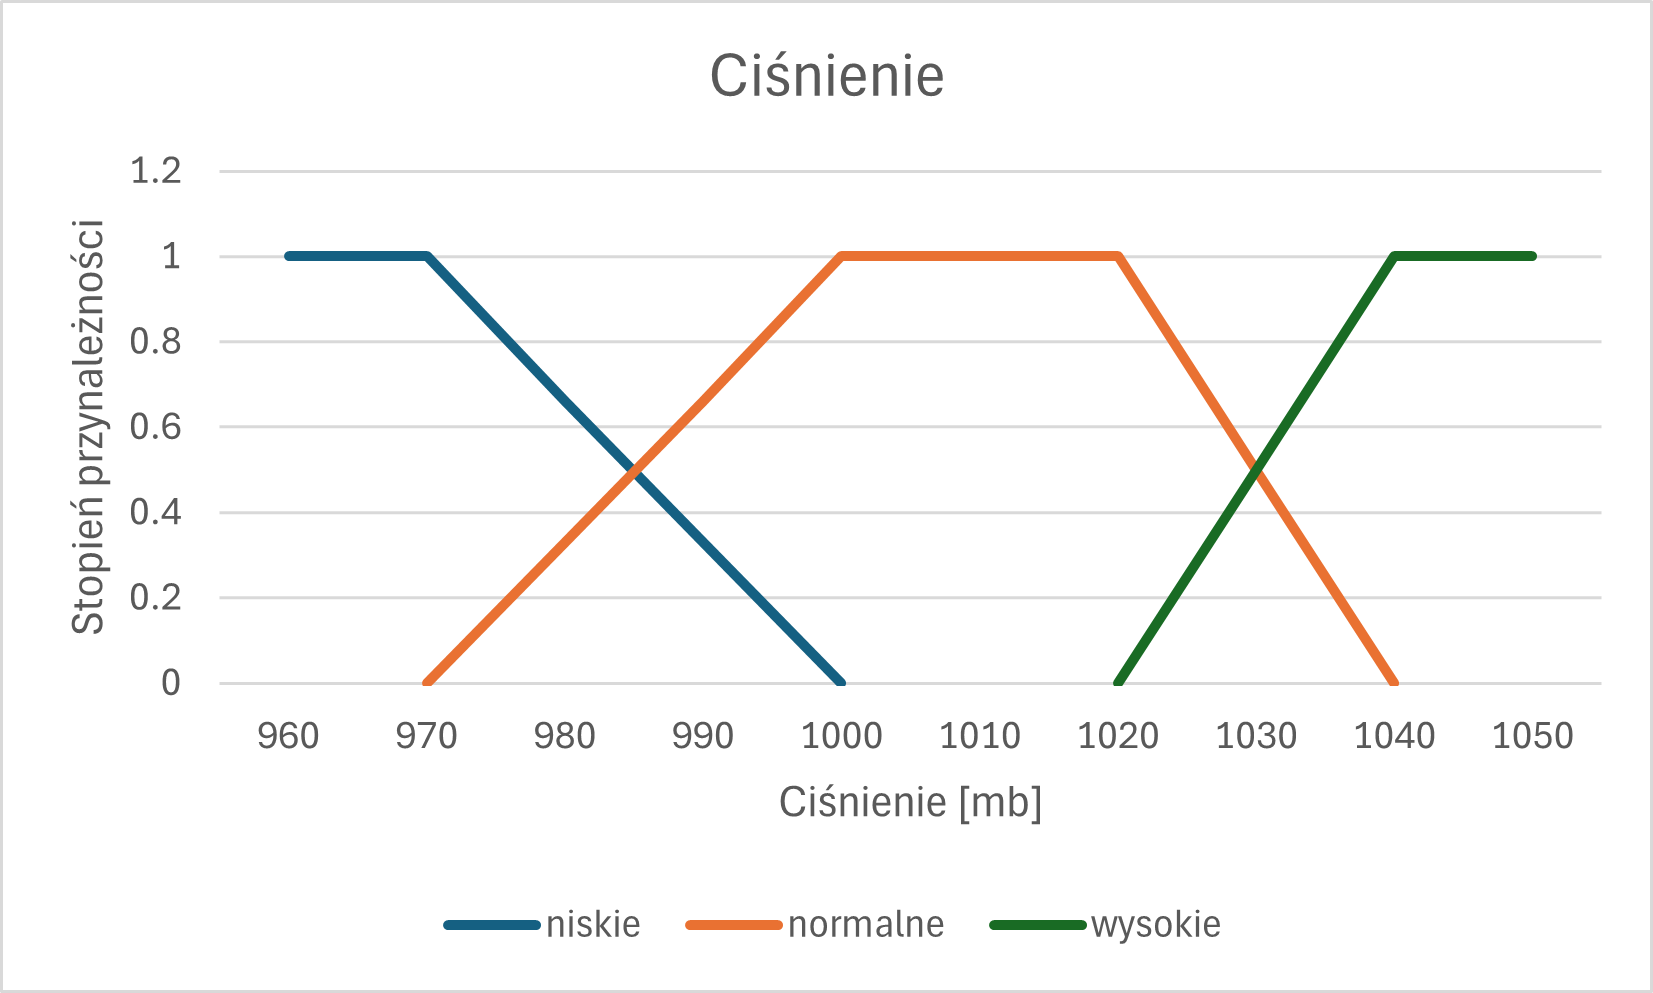
\includegraphics[width=\textwidth]{img/pressure.png}
    \caption{Wykres funkcji przynależności dla ciśnienia.}
    \end{figure}
    
    \item humidity
    \begin{equation}
            L_5 = \langle \mathcal{L}_5, H_5, \mathcal{X}_5 \rangle
        \end{equation}
        gdzie: $\mathcal{L}_5$ – wilgotność powietrza, $H_5$ – \{suche, umiarkowane, wilgotne\}, $\mathcal{X}_1 = [2, 100]$. \\
        Poniżej wzory dla wszystkich możliwych etykiet.

        \begin{equation}
        \mu_{\text{sucho}}(x) =
        \begin{cases}
        1, & x \in (0, 10] \\
        \frac{50 - x}{40}, & x \in (10, 50) \\
        0, & \text{w przeciwnym razie}
        \end{cases}
        \end{equation}

        \begin{equation}
        \mu_{\text{umiarkowane}}(x) =
        \begin{cases}
        \frac{x - 10}{40}, & x \in (10, 50) \\
        1, & x = 50 \\
        \frac{80 - x}{30}, & x \in (50, 80) \\
        0, & \text{w przeciwnym razie}
        \end{cases}
        \end{equation}

        \begin{equation}
        \mu_{\text{wilgotne}}(x) =
        \begin{cases}
        \frac{x - 50}{30}, & x \in (50, 80) \\
        1, & x \in [80, 100] \\
        0, & \text{w przeciwnym razie}
        \end{cases}
        \end{equation}

        \begin{figure}[H]
        \centering
        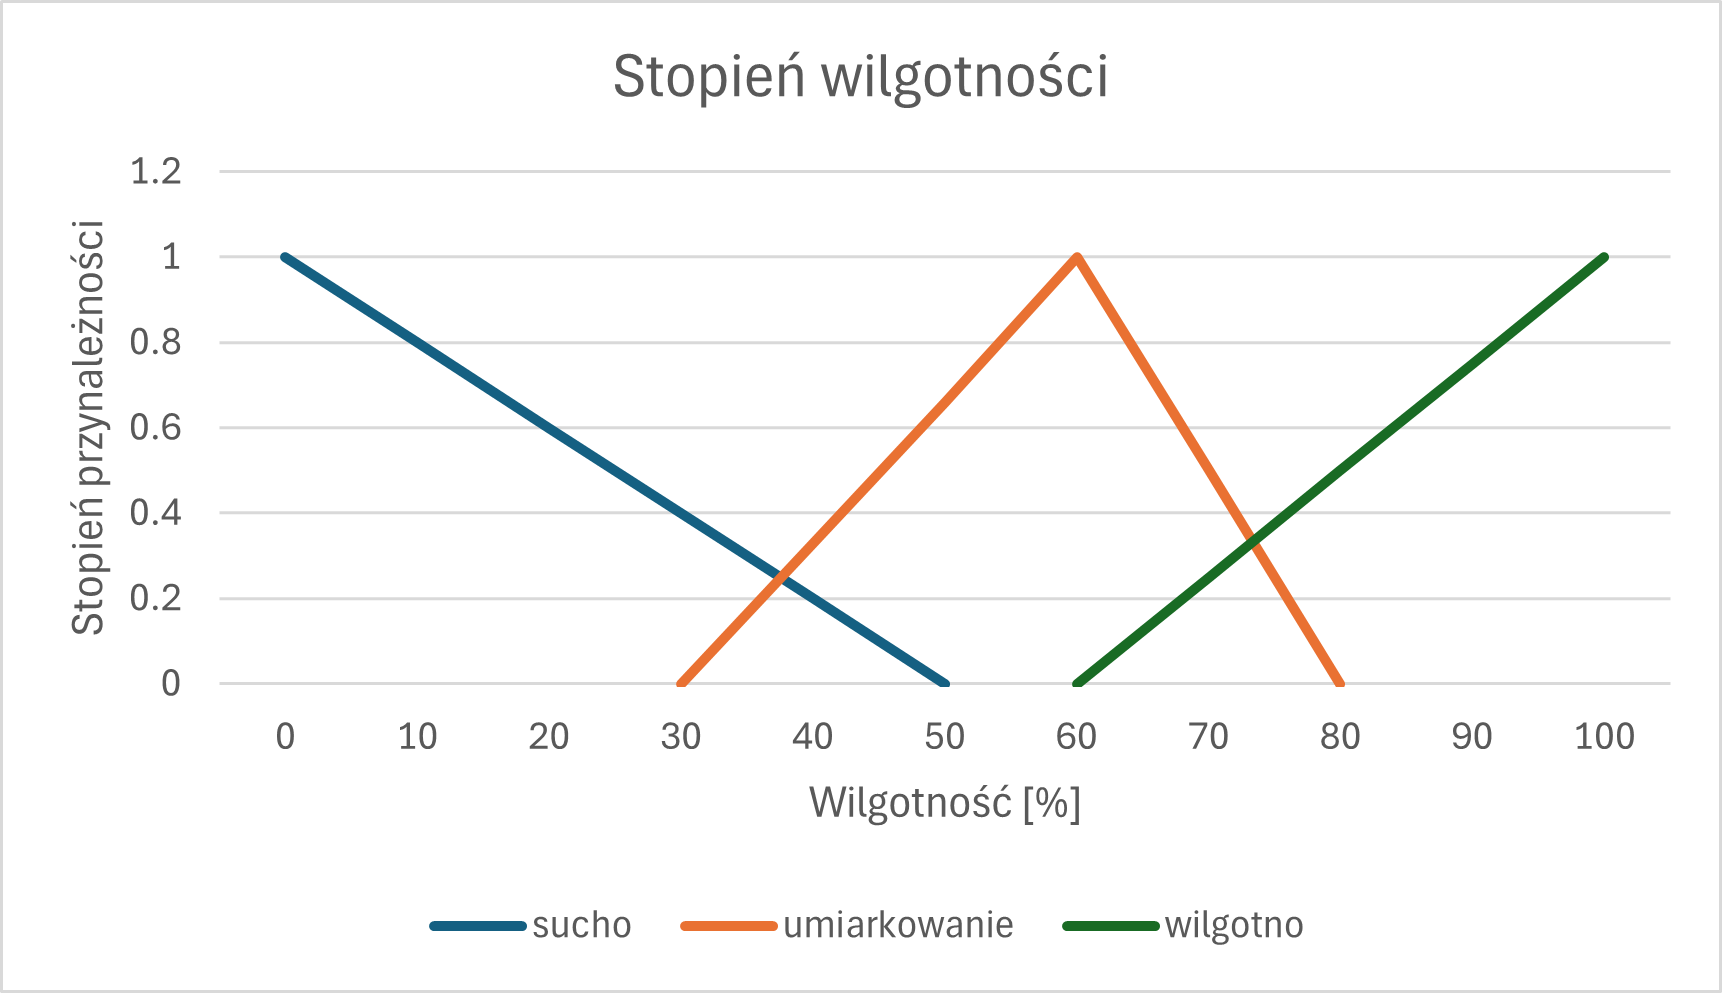
\includegraphics[width=\textwidth]{img/humidity.png}
        \caption{Wykres funkcji przynależności dla stopnia wilgotności.}
        \end{figure}

    \item visibility\_km
    \begin{equation}
            L_6 = \langle \mathcal{L}_6, H_6, \mathcal{X}_6 \rangle
        \end{equation}
        gdzie: $\mathcal{L}_6$ – stopień widoczności, $H_6$ – \{słaba, umiarkowana, dobra, bardzo dobra\}, $\mathcal{X}_6 = [0, 32]$. \\
        Poniżej wzory dla wszystkich możliwych etykiet.
        
    \begin{equation}
    \mu_{\text{słaba}}(x) =
    \begin{cases}
    1, & x \in [0, 4] \\
    \frac{8 - x}{4}, & x \in (4, 8] \\
    0, & \text{w przeciwnym razie}
    \end{cases}
    \end{equation}
    
    \begin{equation}
    \mu_{\text{umiarkowana}}(x) =
    \begin{cases}
    \frac{x - 4}{4}, & x \in (4, 8] \\
    1, & x \in (8, 12] \\
    \frac{16 - x}{4}, & x \in (12, 16] \\
    0, & \text{w przeciwnym razie}
    \end{cases}
    \end{equation}
    
    \begin{equation}
    \mu_{\text{dobra}}(x) =
    \begin{cases}
    \frac{x - 12}{4}, & x \in (12, 16] \\
    1, & x \in (16, 24] \\
    \frac{28 - x}{4}, & x \in (24, 28] \\
    0, & \text{w przeciwnym razie}
    \end{cases}
    \end{equation}

    \begin{equation}
    \mu_{\text{bardzo\_dobra}}(x) =
    \begin{cases}
    \frac{x - 24}{4}, & x \in (24, 28] \\
    1, & x \in (28, 32] \\
    0, & \text{w przeciwnym razie}
    \end{cases}
    \end{equation}

    \begin{figure}[H]
    \centering
    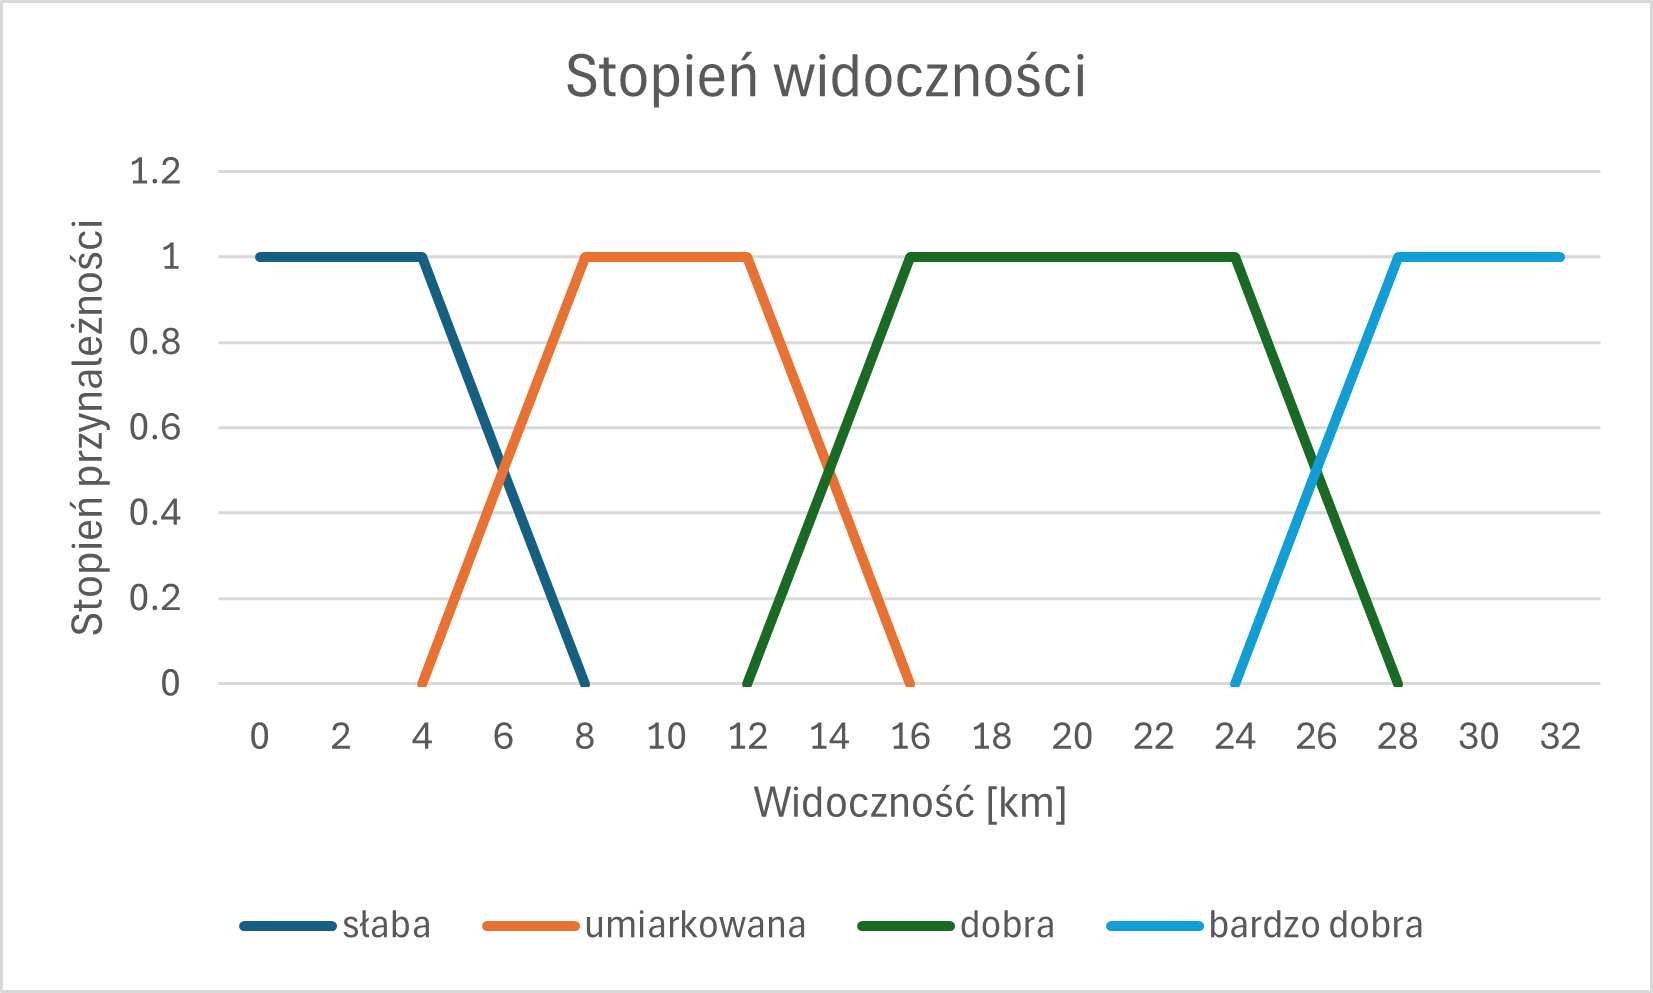
\includegraphics[width=\textwidth]{img/visibility.png}
    \caption{Wykres funkcji przynależności dla stopnia widoczności.}
    \end{figure}

    \item uv\_index
    \begin{equation}
            L_7 = \langle \mathcal{L}_7, H_7, \mathcal{X}_7 \rangle
        \end{equation}
        gdzie: $\mathcal{L}_7$ – promieniowanie UV, $H_1$ – \{niskie, umiarkowane, wysokie, bardzo wysokie, ekstremalne\}, $\mathcal{X}_7 = [0, 16]$. \\
        Poniżej wzory dla wszystkich możliwych etykiet.

    \begin{equation}
    \mu_{\text{niskie}}(x) =
    \begin{cases}
    1, & x \in [0, 2] \\
    \frac{3 - x}{1}, & x \in (2, 3] \\
    0, & \text{w przeciwnym razie}
    \end{cases}
    \end{equation}
    
    \begin{equation}
    \mu_{\text{umiarkowane}}(x) =
    \begin{cases}
    \frac{x - 2}{1}, & x \in (2, 3] \\
    1, & x \in (3, 5] \\
    \frac{6 - x}{1}, & x \in (5, 6) \\
    0, & \text{w przeciwnym razie}
    \end{cases}
    \end{equation}
    
    \begin{equation}
    \mu_{\text{wysokie}}(x) =
    \begin{cases}
    \frac{x - 5}{1}, & x \in (5, 6] \\
    1, & x \in (6, 7] \\
    \frac{8 - x}{1}, & x \in (7, 8) \\
    0, & \text{w przeciwnym razie}
    \end{cases}
    \end{equation}
    
    \begin{equation}
    \mu_{\text{bardzo\_wysokie}}(x) =
    \begin{cases}
    \frac{x - 7}{1}, & x \in (7, 8] \\
    1, & x \in (8, 10] \\
    \frac{11 - x}{1}, & x \in (10, 11) \\
    0, & \text{w przeciwnym razie}
    \end{cases}
    \end{equation}

    \begin{equation}
    \mu_{\text{ekstremalne}}(x) =
    \begin{cases}
    \frac{x - 10}{1}, & x \in (10, 11] \\
    1, & x \in (11, 16] \\
    0, & \text{w przeciwnym razie}
    \end{cases}
    \end{equation}

    \begin{figure}[H]
    \centering
    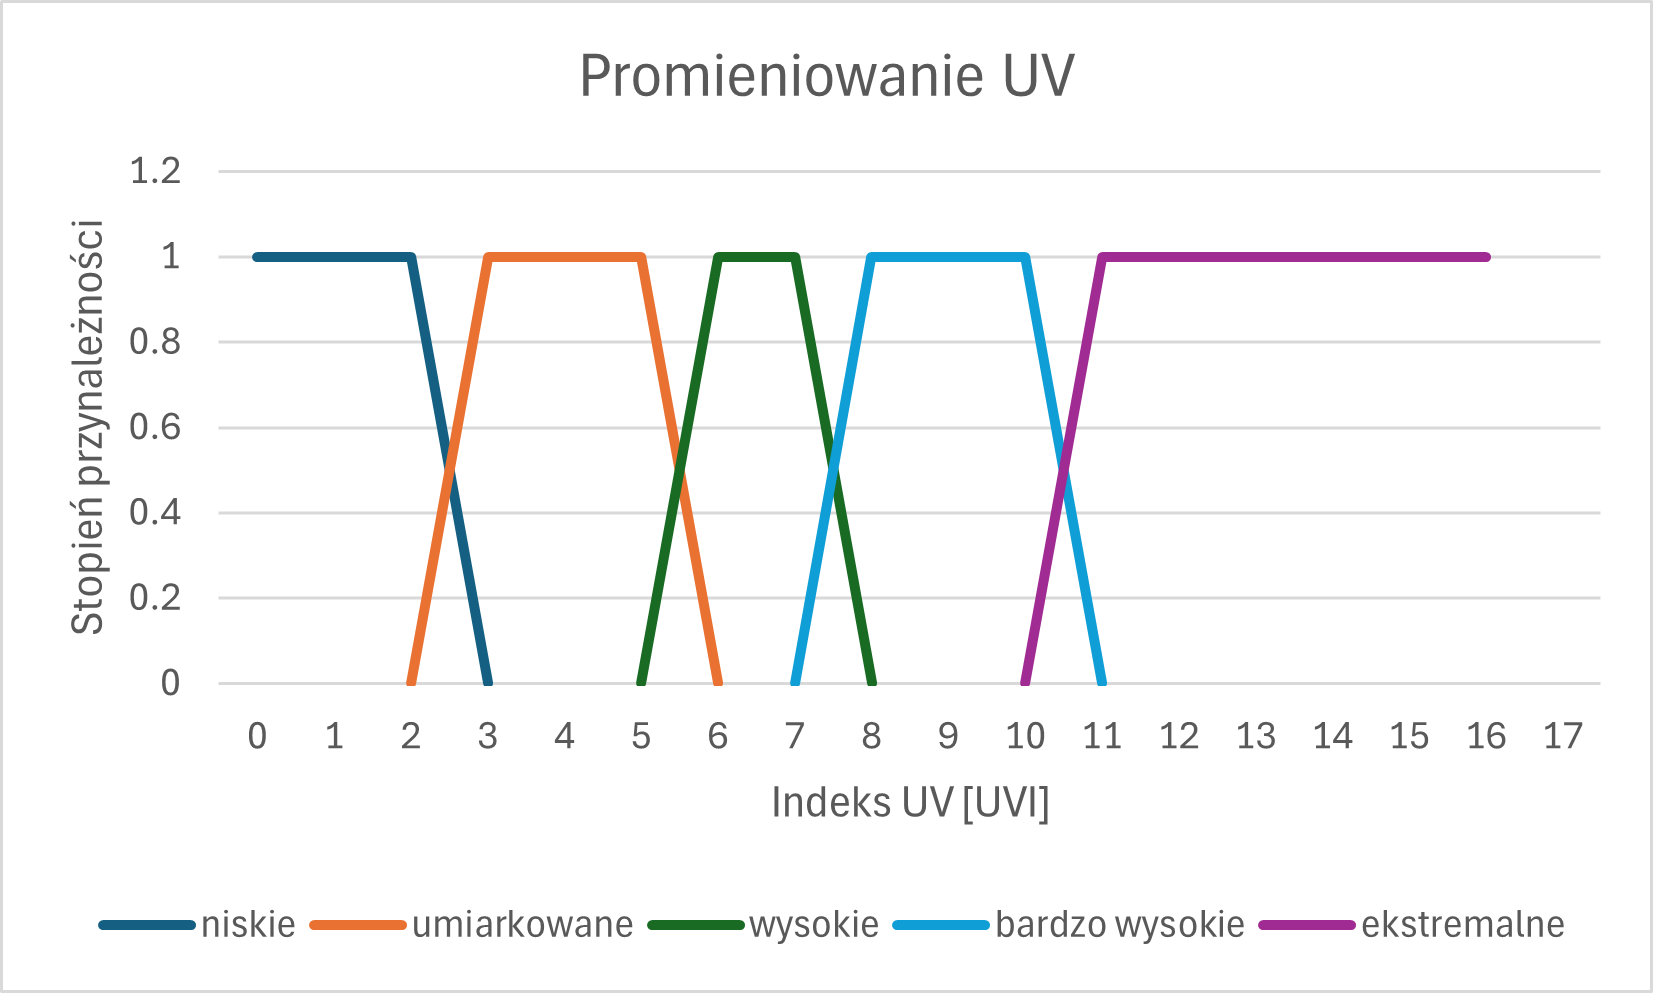
\includegraphics[width=\textwidth]{img/uv.png}
    \caption{Wykres funkcji przynależności dla promieniowania UV.}
    \end{figure}

    \item air\_quality\_Carbon\_Monoxide
            \begin{equation}
            L_8 = \langle \mathcal{L}_8, H_8, \mathcal{X}_8 \rangle
        \end{equation}
        gdzie: $\mathcal{L}_8$ – zanieczyszczenie CO2, $H_8$ – \{normalne, niezdrowe, niebezpieczne\}, $\mathcal{X}_8 = [0, 2220]$. \\
        Poniżej wzory dla wszystkich możliwych etykiet.

    \begin{equation}
    \mu_{\text{normalne}}(x) =
    \begin{cases}
    1, & x \in [0, 200] \\
    \frac{400 - x}{200}, & x \in (200, 400] \\
    0, & \text{w przeciwnym razie}
    \end{cases}
    \end{equation}
    
    \begin{equation}
    \mu_{\text{niezdrowe}}(x) =
    \begin{cases}
    \frac{x - 200}{200}, & x \in (200, 400] \\
    1, & x \in (400, 800] \\
    \frac{1000 - x}{200}, & x \in (800, 1000) \\
    0, & \text{w przeciwnym razie}
    \end{cases}
    \end{equation}
    
    \begin{equation}
    \mu_{\text{niebezpieczne}}(x) =
    \begin{cases}
    \frac{x - 800}{200}, & x \in (800, 1000] \\
    1, & x > \ in (1000, 2220] \\
    0, & \text{w przeciwnym razie}
    \end{cases}
    \end{equation}

    \begin{figure}[H]
    \centering
    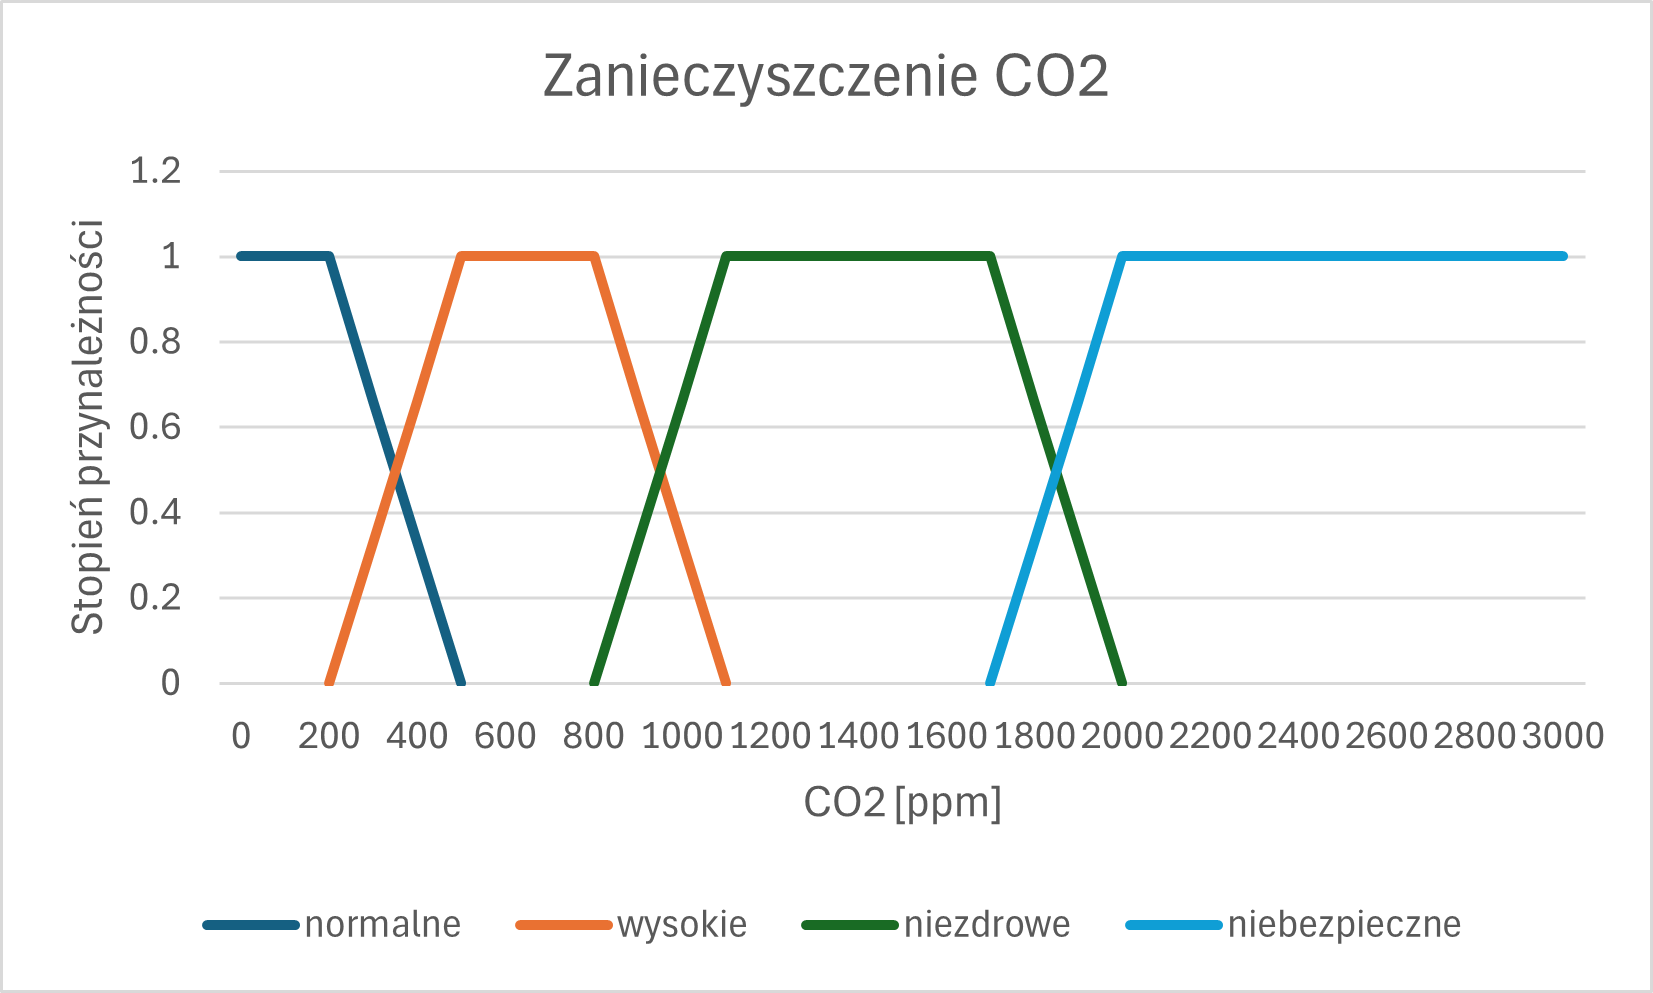
\includegraphics[width=\textwidth]{img/co.png}
    \caption{Wykres funkcji przynależności dla zanieczyszczenia CO2.}
    \end{figure}
    
    \item air\_quality\_Nitrogen\_dioxide
                \begin{equation}
            L_9 = \langle \mathcal{L}_9, H_9, \mathcal{X}_9 \rangle
        \end{equation}
        gdzie: $\mathcal{L}_9$ – zanieczyszczenie NO2, $H_9$ – \{normalne, niezdrowe, niebezpieczne\}, $\mathcal{X}_9 = [0, 428]$. \\
        Poniżej wzory dla wszystkich możliwych etykiet.

    \begin{equation}
    \mu_{\text{normalne}}(x) =
    \begin{cases}
    1, & x \in [0, 50] \\
    \frac{100 - x}{50}, & x \in (50, 100] \\
    0, & \text{w przeciwnym razie}
    \end{cases}
    \end{equation}
    
    \begin{equation}
    \mu_{\text{niezdrowe}}(x) =
    \begin{cases}
    \frac{x - 50}{50}, & x \in (50, 100] \\
    1, & x \in (100, 200] \\
    \frac{250 - x}{50}, & x \in (200, 250) \\
    0, & \text{w przeciwnym razie}
    \end{cases}
    \end{equation}
    
    \begin{equation}
    \mu_{\text{niebezpieczne}}(x) =
    \begin{cases}
    \frac{x - 200}{50}, & x \in (200, 250] \\
    1, & x \in (250, 428] \\
    0, & \text{w przeciwnym razie}
    \end{cases}
    \end{equation}

        \begin{figure}[H]
    \centering
    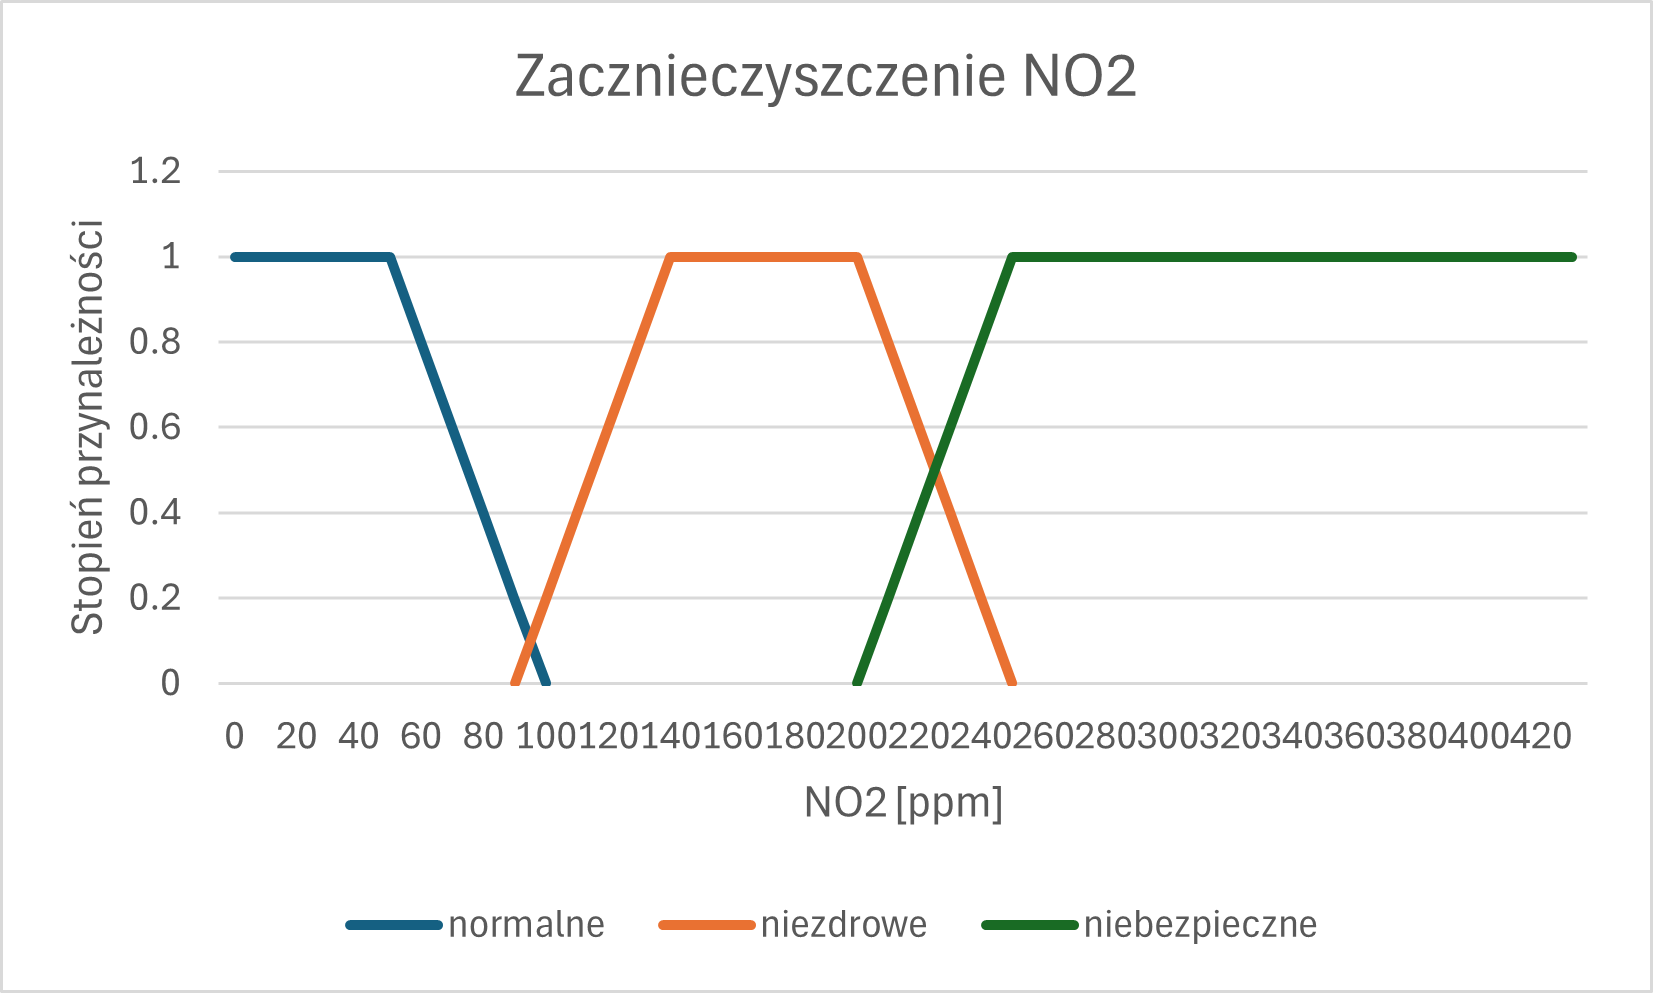
\includegraphics[width=\textwidth]{img/no.png}
    \caption{Wykres funkcji przynależności dla zanieczyszczenia no2.}
    \end{figure}
        
    \item Indeks jakości powietrza
                \begin{equation}
            L_10 = \langle \mathcal{L}_{10}, H_{10}, \mathcal{X}_{10} \rangle
        \end{equation}
        gdzie: $\mathcal{L}_{10}$ – jakość powietrza, $H_{10}$ – \{bardzo dobra, dobra, umiarkowana, zła, bardzo zła\}, $\mathcal{X}_{10} = [1, 10]$. \\
        Poniżej wzory dla wszystkich możliwych etykiet.

\begin{equation}
\mu_{\text{bardzo\_dobra}}(x) =
\begin{cases}
1, & x \in [1, 2] \\
\frac{3 - x}{1}, & x \in (2, 3] \\
0, & \text{w przeciwnym razie}
\end{cases}
\end{equation}

\begin{equation}
\mu_{\text{dobra}}(x) =
\begin{cases}
\frac{x - 2}{1}, & x \in (2, 3] \\
1, & x \in (3, 4] \\
\frac{5 - x}{1}, & x \in (4, 5) \\
0, & \text{w przeciwnym razie}
\end{cases}
\end{equation}

\begin{equation}
\mu_{\text{umiarkowana}}(x) =
\begin{cases}
\frac{x - 4}{1}, & x \in (4, 5] \\
1, & x \in (5, 6] \\
\frac{7 - x}{1}, & x \in (6, 7) \\
0, & \text{w przeciwnym razie}
\end{cases}
\end{equation}  

                \begin{equation}
                    \mu_{\text{zła}}(x) =
                    \begin{cases}
                    \frac{x - 6}{1}, & x \in (6, 7] \\
                    1, & x \in (7, 8] \\
                    \frac{9 - x}{1}, & x \in (8, 9)\\
                    0, & \text{w przeciwnym razie} \\
                    \end{cases}
                \end{equation}

                \begin{equation}
                    \mu_{\text{bardzo zła}}(x) =
                    \begin{cases}
                    \frac{x - 8}{1}, &  x \in (8, 9] \\
                    1, & x \in (9, 10] \\
                    0, & \text{w przeciwnym razie} \\
                    \end{cases}
                \end{equation}

    \begin{figure}[H]
    \centering
    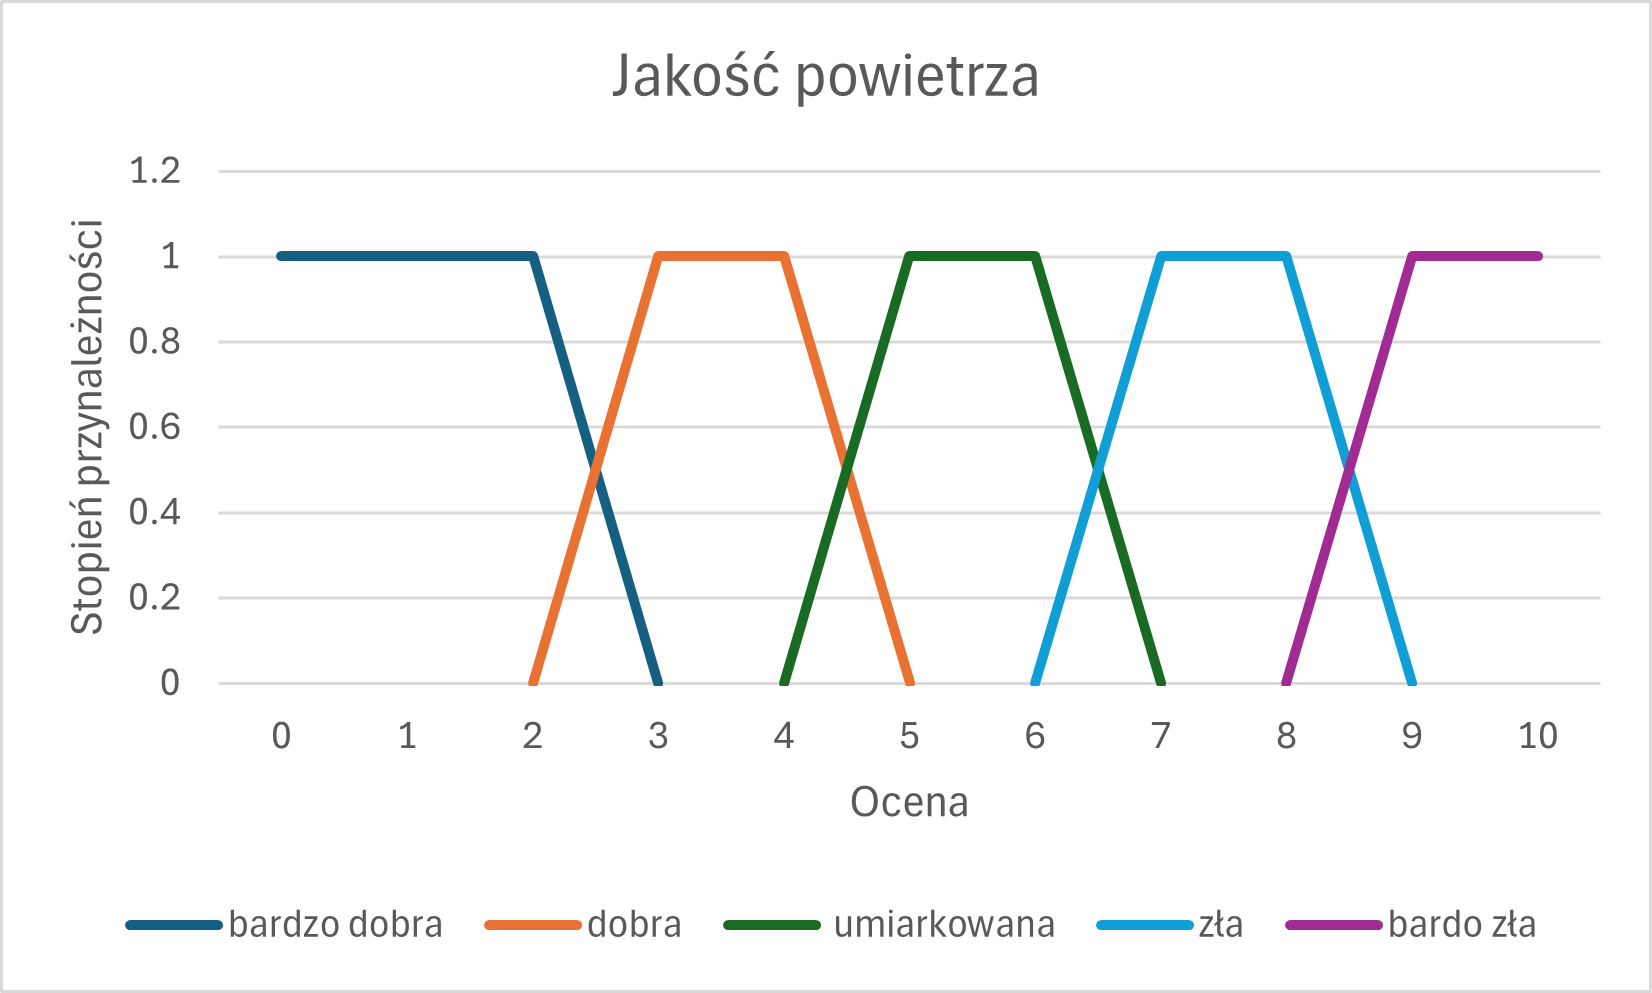
\includegraphics[width=\textwidth]{img/air.png}
    \caption{Wykres funkcji przynależności dla jakości powietrza.}
    \end{figure}
\end{enumerate}

\subsection{Kwantyfikatory lingwistyczne (liczności obiektów)}
Poniżej zostały zaprezentowane kwantyfikatory lingwistyczne wraz z ich wzorami analitycznymi oraz wykresem funkcji przynależności.
\begin{itemize}
    \item[-] prawie żaden
        \begin{equation}
            \mu_{\text{prawie\_żaden}}(x) =
        \begin{cases}
        \exp\left( -\frac{1}{2} \left( \frac{x - 0{,}0}{0,06} \right)^2 \right), & x \in (0, 0.2) \\
        0, & \text{w przeciwnym razie}
        \end{cases}
        \end{equation}
    \item[-] trochę
        \begin{equation}
            \mu_{\text{trochę}}(x) =
            \begin{cases}
            \frac{x - 0.10}{0.15}, & x \in (0.10, 0.25) \\
            1, & x \in [0.25, 0.30] \\
            \frac{0.45 - x}{0.15}, & x \in (0.30, 0.45)\\
            0, & \text{w przeciwnym razie} \\
            \end{cases}
        \end{equation}
    \item[-] około połowa
        \begin{equation}
        \mu_{\text{około połowa}}(x) =
        \begin{cases}
        \exp\left( -\frac{1}{2} \left( \frac{x - 0{,}5}{0,06} \right)^2 \right), & x \in (0.35, 0.75) \\
        0, & \text{w przeciwnym razie}
\end{cases}
        \end{equation}
    \item[-] wiele
        \begin{equation}
             \mu_{\text{trochę}}(x) =
            \begin{cases}
            \frac{x - 0.60}{0.15}, & x \in (0.60, 0.75) \\
            1, & x \in [0.75, 0.80] \\
            \frac{0.95 - x}{0.15}, & x \in (0.80, 0.95)\\
            0, & \text{w przeciwnym razie} \\
            \end{cases}
        \end{equation}
    \item[-] prawie wszystkie
        \begin{equation}
            \mu_{\text{prawie wszystkie}}(x) =
            \begin{cases}
            \exp\left( -\frac{1}{2} \left( \frac{x - 1{,}0}{0,06} \right)^2 \right), &  x \in (0.8, 1.0) \\
            0, & \text{w przeciwnym razie}
            \end{cases}
        \end{equation}
\end{itemize}

\begin{figure}[H]
\centering
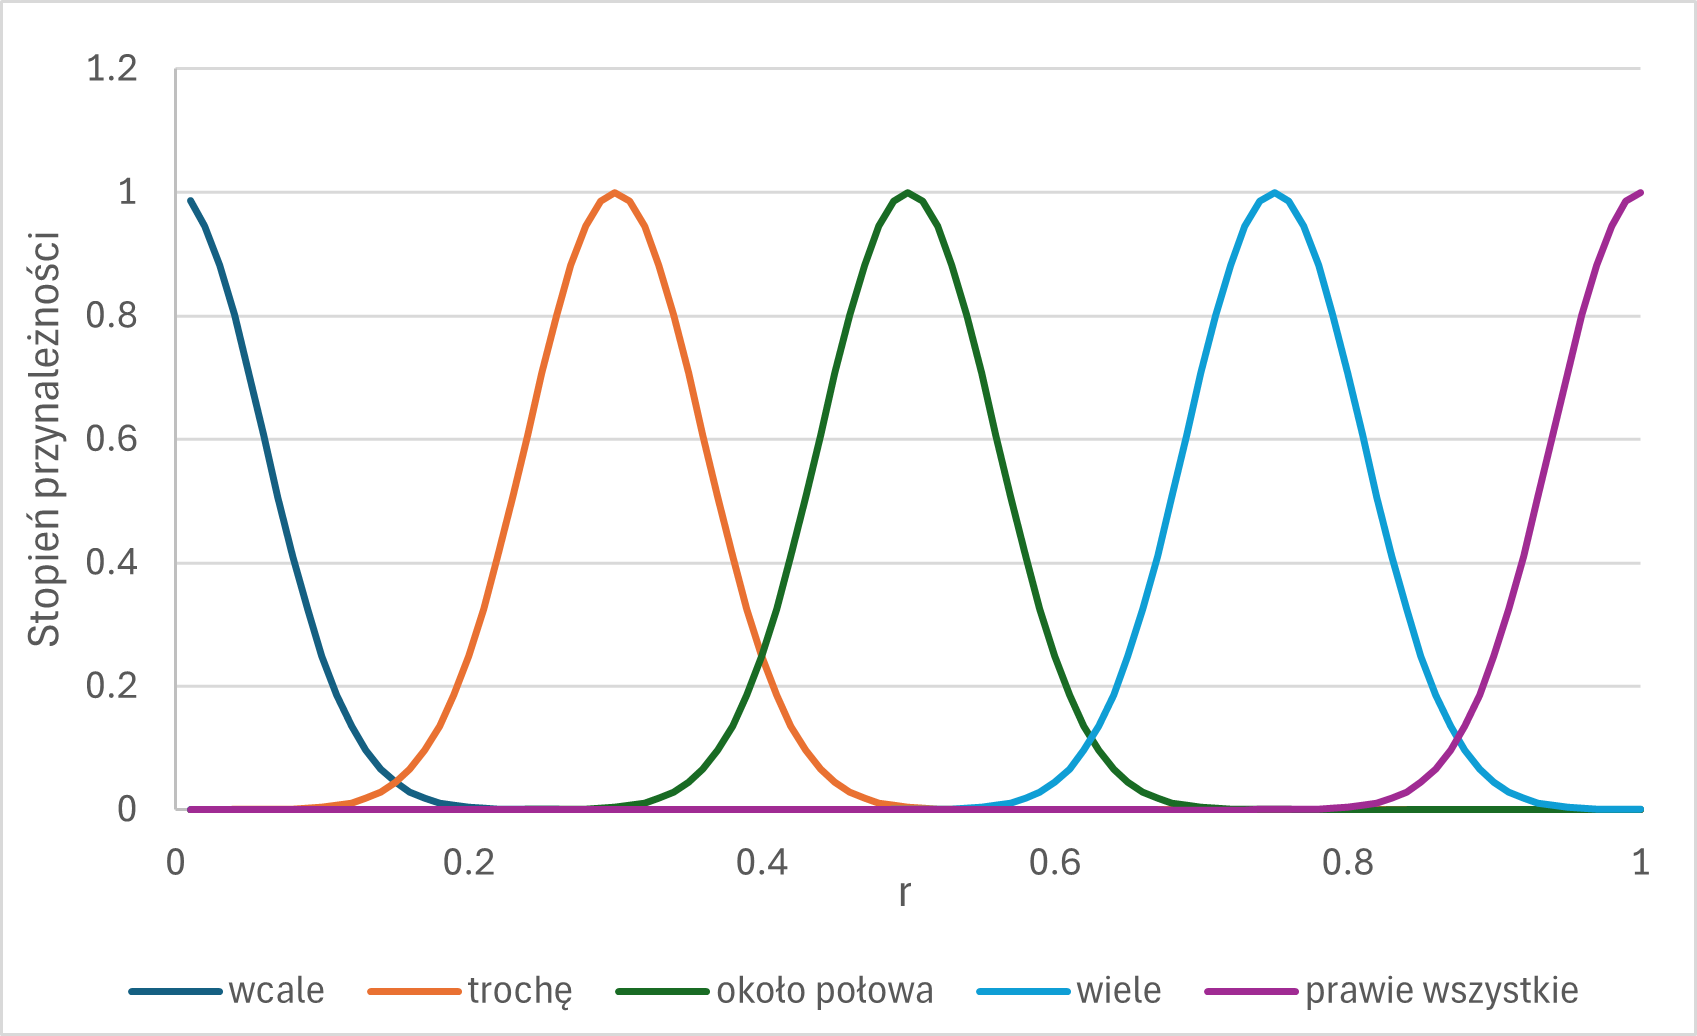
\includegraphics[width=\textwidth]{img/a.png}
\caption{Funkcja przynależności dla wybranych kwantyfikatorów lingwistycznych.}
\end{figure}


\section{Narzędzia obliczeniowe: wybór/implementacja. Diagram UML klas do obliczeń rozmytych i generowania podsumowań}
Program został napisany w języku Java w wersji JDK 24. Do obsługi relacyjnej bazy danych PostgreSQL wykorzystano framework Spring Boot, który umożliwia wygodną konfigurację połączenia z bazą danych. Kod źródłowy komponentu odpowiedzialnego za obliczenia rozmyte został umieszczony w pakiecie o nazwie \texttt{fuzzy}. Znajduje sie w nim podstawowy model reprezentujący zbiory rozmyte, którego centralnym elementem jest abstrakcyjna klasa \texttt{FuzzySet}, która definiuje fundamentalne operacje na zbiorach rozmytych. Klasa ta udostępnia metody pozwalające na obliczanie podstawowych właściwości zbioru rozmytego, m.in. takich jak kardynalność oraz nośnik. Na bazie klasy \texttt{FuzzySet} zbudowane zostały trzy klasy reprezentujące konkretne typy funkcji przynależności: \texttt{GaussianFunction}, \texttt{TrapezoidalFunction} oraz \texttt{TriangularFunction}. Każda z tych klas implementuje matematyczną funkcję przynależności o charakterystycznym kształcie: odpowiednio gaussowskim, trapezoidalnym i trójkątnym. Dzięki temu możliwe jest precyzyjne modelowanie różnych pojęć językowych. \\
Oprócz modelu zbiorów rozmytych, pakiet \texttt{fuzzy} zawiera również klasy odpowiedzialne za tworzenie i przetwarzanie podsumowań lingwistycznych. Klasa \texttt{LinguisticVariable} reprezentuje zmienną lingwistyczną, która zawiera nazwę, przestrzeń rozważań oraz zestaw powiązanych z nią terminów lingwistycznych, np. „bardzo zimno”, „ciepło”, „gorąco”, które są reprezentowane przez odpowiednie zbiory rozmyte.
W strukturze podsumowań lingwistycznych wyróżniamy także kwalifikatory i sumaryzatory, które mają bardzo podobną strukturę, ponieważ są złożone z nazwy oraz przypisanego im zbioru rozmytego. Ich różnice wynikają jedynie z zastosowania, w jaki sposób są wykorzystywane w podsumowaniach lingwistycznych. W celu zachowania przejrzystości i uniknięcia duplikacji kodu, stworzona została wspólna klasa bazowa \texttt{LinguisticTerm}, z której dziedziczą klasy \texttt{Qualifier} oraz \texttt{Summarizer}. Pozwala to na zachowanie semantycznego rozróżnienia przy jednoczesnym wykorzystaniu wspólnej logiki przetwarzania.
Klasa \texttt{Quantifier} odpowiada za reprezentację kwantyfikatorów, takich jak „około połowy” czy „prawie żaden”. Kwantyfikator opisany jest za pomocą nazwy, funkcji przynależności oraz typu — może być kwantyfikatorem absolutnym lub względnym.
Ostatnim elementem pakietu jest klasa \texttt{Summary}. To ona odpowiada za generowanie podsumowań lingwistycznych na podstawie przekazanych obiektów: sumaryzatora, kwalifikatora oraz kwantyfikatora. \\
Strukturę logiczną opisanych klas oraz zależności między nimi przedstawiono na poniższym diagramie UML.


\begin{figure}[H]
\centering
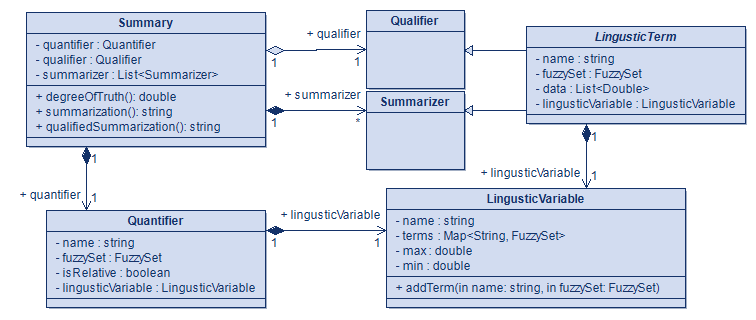
\includegraphics[width=\textwidth]{img/lingustic.png}
\caption{Diagram UML pakietu \texttt{fuzzy}.}
\end{figure}


\section{ Jednopodmiotowe podsumowania lingwistyczne. Miary jakości, podsumowanie optymalne}
Wyniki kolejnych eksperymentów wg punktów 2.-4. opisu projektu 2.  Listy podsumowań
jednopodmiotowych i tabele/rankingi podsumowań dla danych atrybutów obowiązkowe i dokładnie opisane w ,,captions'' (tytułach), konieczny opis kolumn i wierszy tabel. Dla każdego podsumowania podane miary jakości oraz miara jakości podsumowania
optymalnego. {\bf Wzorów podsumowań ani miar nie należy przepisywać ani cytować, wystarczy podać literaturę, ale
należy skomentować co oznaczają i jaką informacje niosą wybrane miary w wybranych
przypadkach.}\\
\noindent {\bf Sekcja uzupełniona jako efekt zadania Tydzień 11 wg Harmonogramu Zajęć na WIKAMP KSR.}

\section{Wielopodmiotowe podsumowania lingwistyczne i~ich miary jakości} 
Wyniki kolejnych eksperymentów wg punktów 2.-4. opisu projektu 2. Uzasadnienie i
metoda podziału zbioru danych na rozłączne podmioty. Listy podsumowań
wielopodmiotowych i tabele/rankingi podsumowań dla danych atrybutów obowiązkowe i
dokładnie opisane w ,,captions'' (tytułach), konieczny opis kolumn i wierszy tabel.
{\bf Wzorów podsumowań ani miar nie należy przepisywać ani cytować, wystarczy podać literaturę, ale
należy skomentować co oznaczają i jaką informacje niosą wybrane miary w wybranych
przypadkach.} Konieczne uwzględnienie wszystkich 4-ch form podsumowań wielopodmiotowych. 
\\ 

** Możliwe sformułowanie zagadnienia wielopodmiotowego podsumowania optymalnego **.\\
\indent {** Ewentualne wyniki realizacji punktu ,,na ocenę 5.0'' wg opisu Projektu 2. i ich porównanie do wyników z
części obowiązkowej **.}\\

\noindent {\bf Sekcja uzupełniona jako efekt zadania Tydzień 12 wg Harmonogramu Zajęć
na WIKAMP KSR.}


\section{Dyskusja, wnioski}
Dokładne interpretacje uzyskanych wyników w zależności od parametrów klasyfikacji
opisanych w punktach 3.-4 opisu Projektu 2. 
Omówić i wyjaśnić napotkane problemy (jeśli były). Każdy wniosek/problem powinien mieć poparcie
w przeprowadzonych eksperymentach (odwołania do konkretnych wyników: tabel i miar
jakości). Ocena które podsumowania i dlaczego niosą najistotniejsze informacje
i które ich miary jakości mają małe albo duże znaczenie dla wiarygodności i jakości otrzymanych
agregacji/podsumowań.  \\
\underline{Dla końcowej oceny jest to najważniejsza sekcja} sprawozdania, gdyż prezentuje poziom
zrozumienia rozwiązywanego problemu.\\

** Możliwości kontynuacji prac w obszarze logiki rozmytej i wnioskowania rozmytego, zwłaszcza w kontekście pracy inżynierskiej,
magisterskiej, naukowej, itp. **\\

\noindent {\bf Sekcja uzupełniona jako efekt zadań Tydzień 11 i Tydzień 12 wg
Harmonogramu Zajęć na WIKAMP KSR.}


\section{Braki w realizacji projektu 2.}
Wymienić wg opisu Projektu 2. wszystkie niezrealizowane obowiązkowe elementy projektu, ewentualnie
podać merytoryczne (ale nie czasowe) przyczyny tych braków. 


\begin{thebibliography}{99}
\bibitem{baza} World Weather Repository - kaggle, \url{https://www.kaggle.com/datasets/nelgiriyewithana/global-weather-repository?resource=download}. [dostęp 18.05.2025r.]
 \bibitem{niewiadomski19} A. Niewiadomski, Zbiory rozmyte typu 2. Zastosowania w reprezentowaniu informacji.  Seria „Problemy współczesnej informatyki” pod redakcją L. Rutkowskiego. Akademicka Oficyna Wydawnicza EXIT, Warszawa, 2019.
\bibitem{zadrozny06} S. Zadrożny, Zapytania nieprecyzyjne i lingwistyczne podsumowania baz danych, EXIT, 2006, Warszawa
\bibitem{niewiadomski08} A. Niewiadomski, Methods for the Linguistic Summarization of Data: Applications of Fuzzy Sets and Their Extensions, Akademicka Oficyna Wydawnicza EXIT, Warszawa, 2008.
\end{thebibliography}

Literatura zawiera wyłącznie źródła recenzowane i/lub o potwierdzonej wiarygodności,
możliwe do weryfikacji i cytowane w sprawozdaniu. 
\end{document}
